\documentclass[a4paper,10pt]{article}

\usepackage{geometry}
%\geometry{a4paper,left=2.5cm,right=2cm,top=3cm,bottom=2cm}

\usepackage[utf8x]{inputenc}
\usepackage[bookmarks,colorlinks=false,pdfborder={0 0 0}]{hyperref}
\hypersetup{pdftitle={3. Praktikum: Modellierung von Informationssystemen}}
\usepackage{url}
\usepackage[ngerman]{babel}
\usepackage{graphicx}
\usepackage{listings}

\parindent 0pt 
\parskip 10pt

\title{3. Praktikum: Modellierung von Informationssystemen}
\author{Andreas Krohn \and Benjamin Vetter \and Erik Andresen \and Jan Depke}

\begin{document}

\maketitle

\tableofcontents

\section{Analyse}

\emph{Welcher konkreter Konfigurator soll re-implementiert werden?}

http://carconfig.toyota-europe.com/

\emph{Welche Schwachstellen sollen in der neuen Fassung vermieden werden?}

\begin{itemize}
 \item Auswahl des Modells soll in dem Konfigurator selbst möglich sein
 \item Wizard - Schrittweises Konfigurieren des Autos
 \item Menü rechts oben.. Sprechendere Namen, nähere Angaben $\rightarrow$ Pro Option eine Seite im Wizard
\end{itemize}

\emph{Welche Fahrzeuggrundtypen gibt?}

\begin{tabular}{|l|}
\hline
Name \\
\hline
iQ \\
AYGO \\
Yaris \\
Urban Cruiser \\
Auris \\
Verso \\
Avensis \\
RAV4 \\
Prius \\
Land Cruiser \\
Land Cruiser V8 \\
\hline
\end{tabular}

\emph{Was ist konfigurierbar?}

\emph{Welche Komponenten sind miteinander verbaubar?}

\section{Design}

\subsection*{Architekturmodell}

Wir haben eine Trennung von Frontend (Präsentationsschicht für Anwender) und Backend (Regelsystem) vorgenommen.
Die Komponenten kommunzieren über ein HTTP-Ähnliches Protokoll.

\subsubsection{Protokoll}
Das Frontend schickt:

\begin{lstlisting}
GET Liste von bereits gewaehlten, alphanumerischen Options-IDs
\end{lstlisting}

z.B.

\begin{lstlisting}
GET yaris,three_doors
\end{lstlisting}

Das Backend antwortet, indem ein \textit{OK} und eine Liste von Options-IDs zurückgegeben wird, die kompatibel mit den empfangen Options-IDs sind.

\begin{lstlisting}
OK benziner,becker_radio,jvc_radio,...
\end{lstlisting}

Nach der Request-Methode (GET, OK, ERR) folgt ein Leerzeichen (ASCII-Wert 0x20). Elemente in der Liste werden durch ein Komma (ASCII-Wert 0x2C) getrennt.
Jeder Request wird durch ein Carriage Return vor einem Newline abgeschlossen. (ASCII 0x0D 0x0A).

\begin{figure}[htb]
	\centering
	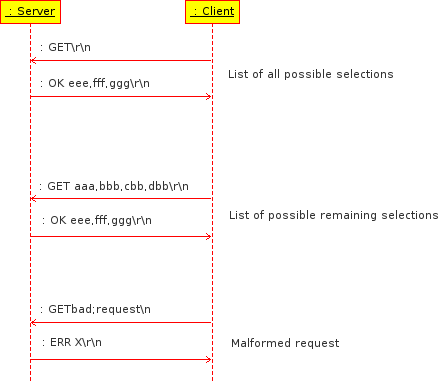
\includegraphics[width=0.6\textwidth]{doc/netsequence.png}
	\caption{Netzwerkprotokoll Sequenzdiagramm}
	\label{fig:networkproto_sequence}
\end{figure}

\subsection*{Arbeitspakete und Zuständigkeiten}

Das Frontend wurde von Andreas Krohn und Benjamin Vetter bearbeitet.
Das Backend wurde von Jan Depke und Erik Andresen bearbeitet.
 
\subsection*{Regelsystem}

\begin{itemize}
 \item Es gibt eine Sequenz von Kategorien (Chassis $\rightarrow$ Reifen $\rightarrow$ Lack $\rightarrow$ \ldots)
 \item Es gibt eine Menge aktuell gewählter Optionen (und - implizit? - abgearbeteter Kategorien), die aktuelle \emph{Konfiguration}
 \item Zu einer Konfiguration liefert das Regelwerk eine Menge noch verfügbarer Kategorien sowie jeweils wählbarer Optionen.
\end{itemize}

\subsection*{Klassenmodell / DB}

\begin{itemize}
 \item Es gibt eine Klasse \emph{Option} (mögl. Ausprägungen: Chassis "`Yaris"', Michelin Reifen "`XYZ"', Metallic-Lackierung "`Schwarz"'\ldots)
 \item Eine Option hat einen Identifier und gehört zu einer \emph{Kategorie} (z.B. Radio, Dachfenster, Bereifung)
 \item Pro Option gibt es eine Liste von Identifiern, mit denen sie kombinierbar ist.
\end{itemize}

Das Frontend (Ruby on Rails) umfasst die Modelle \textit{Option} und \textit{Category}.

\begin{center}
  \begin{figure}[t]
    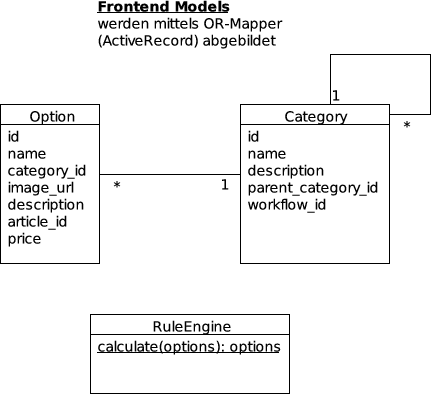
\includegraphics[width=0.7\textwidth]{doc/frontend_models.png}
    \caption{Modelle des Frotends}
    \label{frontend_models}
  \end{figure}
\end{center}

Die Modelle werden mittels OR-Mapper des Frameworks (ActiveRecord) in einer SQLite-Datenbank gespeichert und bedürfen daher keiner weiteren Erläuterungen.
Zusätzlich gibt es ein Modell \textit{RuleEngine}, dass für die Kommunikation mit dem Backend zuständig ist.

Der funktionale Teil des Frontends besteht aus der Klasse \textit{WorkflowController}, der ein Wizard implementiert mit dem der Anwender konfrontiert wird und sein Auto konfigurieren muss (vgl. Screenshots).

\subsection*{GUI}

Im folgenden sind einige Screenshots unserer webbasierten GUI zu sehen.

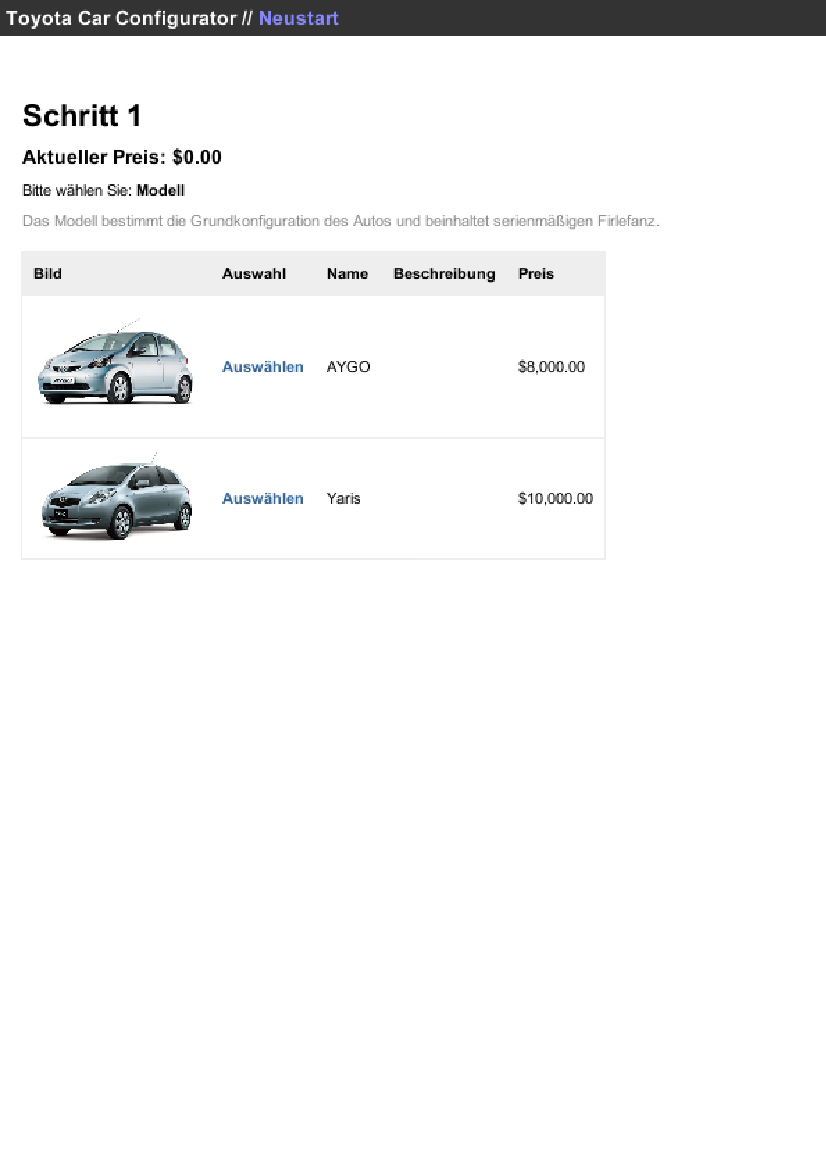
\includegraphics[width=0.8\textwidth]{screenshots/screenshot1.png}
\\
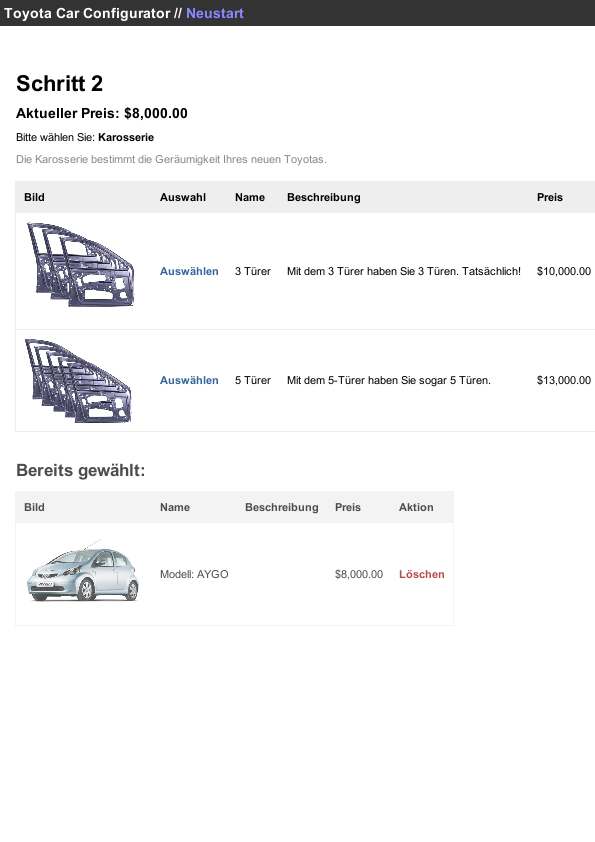
\includegraphics[width=0.8\textwidth]{screenshots/screenshot2.png}
\\
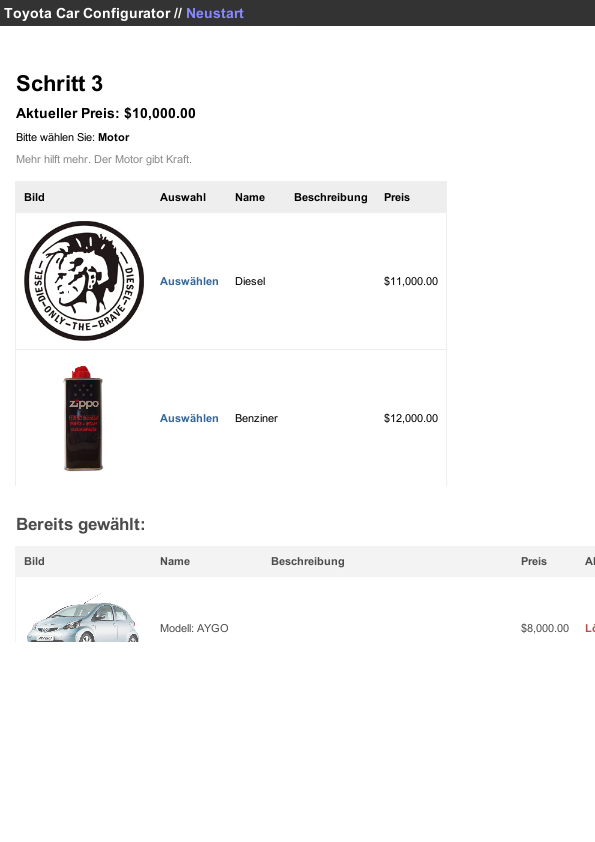
\includegraphics[width=0.8\textwidth]{screenshots/screenshot4.png}
\\
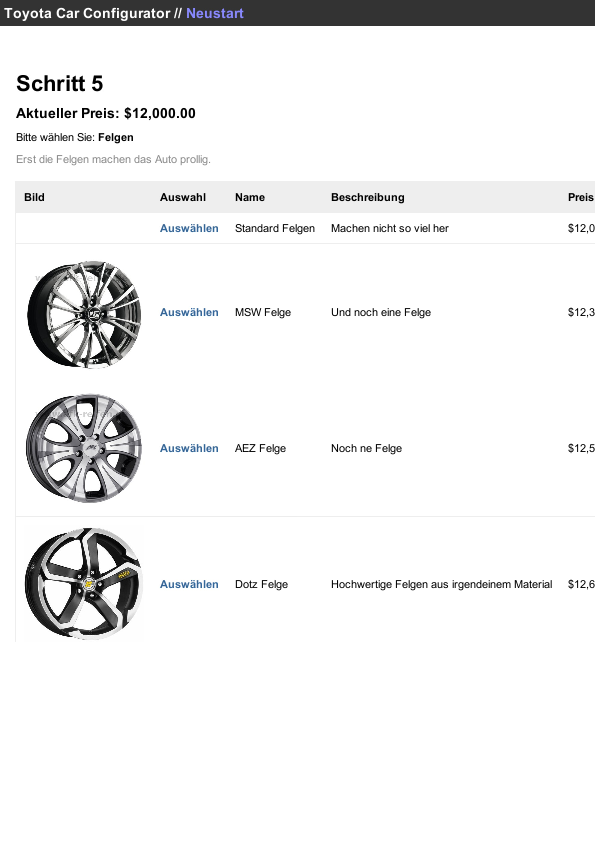
\includegraphics[width=0.8\textwidth]{screenshots/screenshot5.png}
\\
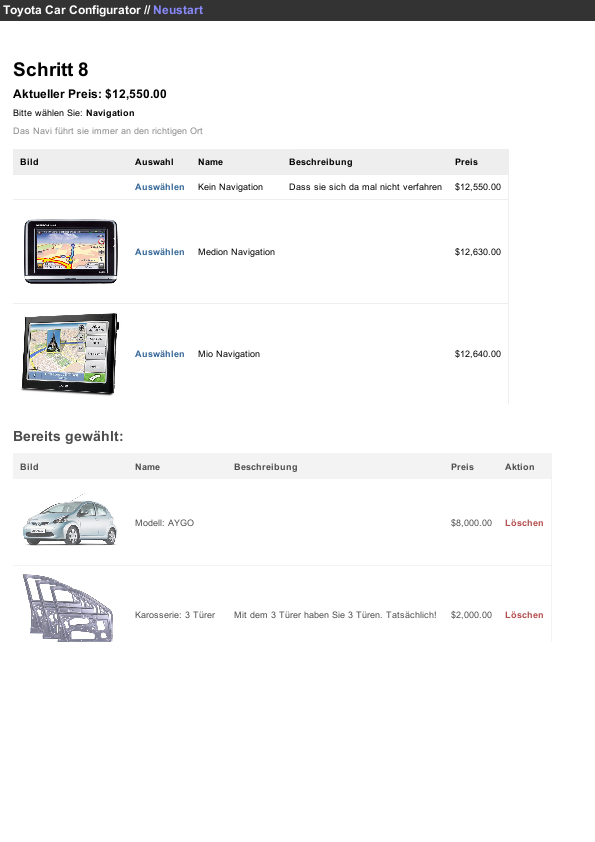
\includegraphics[width=0.8\textwidth]{screenshots/screenshot6.png}
\\
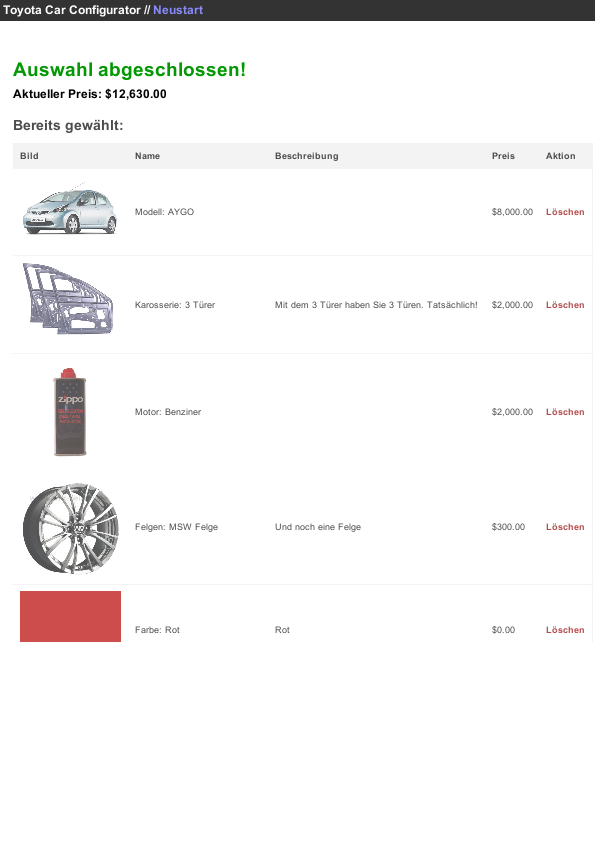
\includegraphics[width=0.8\textwidth]{screenshots/screenshot7.png}

\section{Implementierung}

Für das Frontend wurde \textbf{Ruby on Rails 2.3.5} mit einer SQLite-Datenbank verwendet.
Die GUI ist dementsprechend webbasiert.
Das Backend (Regelsystem) wurde in Java realisiert. 

\section{Tests}

\subsection{Frontend}

Für das Frotend wurden Unit-Tests und Functional-Tests erstellt (vgl. /frontend/test/unit).
Die Unit-Tests testen die Abfragen an das Regelsystem.
Unit-Tests für die Modelle \textit{Option} und \textit{Category} wurden nicht über die automatisch generierten Tests hinaus erstellt, da die Models keinen applikationsspezifischen Code aufweisen.
Die Functional-Tests testen den \textit{WorkflowController} (vgl. /frontend/test/functional).

Das Test-Protokoll für das Frontend:

\begin{lstlisting}
$ rake test
/usr/bin/ruby1.8 -I"lib:test" "/usr/lib/ruby/1.8/rake/rake_test_loader.rb" "test/unit/rule_engine_test.rb" "test/unit/option_test.rb" "test/unit/category_test.rb" "test/unit/helpers/options_helper_test.rb" "test/unit/helpers/categories_helper_test.rb" "test/unit/helpers/workflow_helper_test.rb" 
Loaded suite /usr/lib/ruby/1.8/rake/rake_test_loader
Started
....
Finished in 0.049247 seconds.

4 tests, 4 assertions, 0 failures, 0 errors
/usr/bin/ruby1.8 -I"lib:test" "/usr/lib/ruby/1.8/rake/rake_test_loader.rb" "test/functional/options_controller_test.rb" "test/functional/workflow_controller_test.rb" "test/functional/categories_controller_test.rb" 
Loaded suite /usr/lib/ruby/1.8/rake/rake_test_loader
Started
....................
Finished in 0.264087 seconds.

20 tests, 31 assertions, 0 failures, 0 errors
/usr/bin/ruby1.8 -I"lib:test" "/usr/lib/ruby/1.8/rake/rake_test_loader.rb"  
\end{lstlisting}

\subsection{Backend}
Für das Backend existiert ein Python-Skript nettest/nettest.py das alle möglichen Kombinationen in mehreren Threads durchtestet.

\section{Komponenten/Schnittstellen}

\subsection*{Regelengine}

Aktion:
 

Parameter:
 Liste von (bereits gewählten) Optionen

Rückgabe:
 Liste von wählbaren Optionen

\subsection*{Datenbank}


\section{sonstiges\ldots}
\begin{itemize}
 \item Modelldatenbank
 \item Teile und Konfigurationsoptionen (Farbe, etc..) in DB
 \item Kombinierbarkeit/Konfigurierbarkeit/Regeln in XML-Dateien (die dann Modelle/Teile.. referenzieren)
 \item Verbaubarkeitsregeln in gesondertem Editor?
 \item Ausblick: Workflow/Ablauf konfigurierbar
\end{itemize}

\section{Aufgabe 4 (Prozessmodellierung Auto-Konfigurator)}

\subsection*{Modellierung des Gesamtprozesses in BPMN}

\subsection*{Integration einer Prozess-Engine in unsere Implementierung}

Da wir Probleme mit dem XML-Export aus Activiti heraus haben, haben wir eine YAML-Konfigurationsdatei\footnote{vgl. \url{http://de.wikipedia.org/wiki/YAML}} verwendet, um den Prozess dynamisch anpassbar zu halten.
Die Konfigurationsdatei ist unter /frontend/config/workflow.yml zu finden.
Die Datei spezifiziert die Reihenfolge in der das Wizard durchlaufen wird.

Beispiel bzgl. der Umkonfiguration:

\begin{lstlisting}[numbers=left]
  workflow:
    - modell: 
      - modell 
    - karosserie: 
      - karosserie
    - motor:
      - motor
    - aussenausstattung: 
      - farbe 
      - felgen
    - innenausstattung: 
      - radio 
      - klimaanlage
      - navigation
\end{lstlisting}

Dieses Beispiel spezifiziert, dass nachdem das Modell gewählt wurde, die Karosserie (Türen) gewählt werden muss (siehe Screenshots).

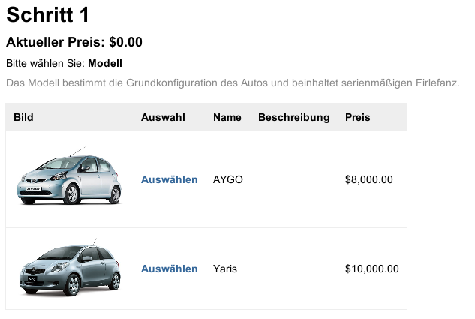
\includegraphics[width=0.8\textwidth]{screenshots/sequence1.png}
\\
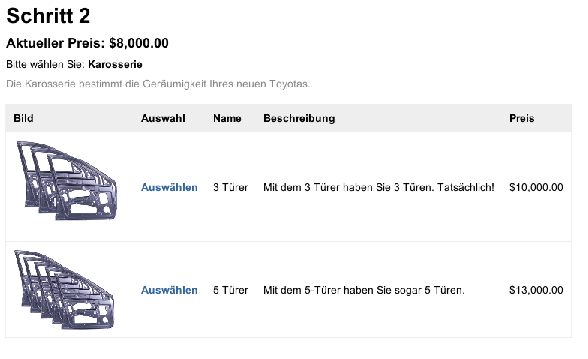
\includegraphics[width=0.8\textwidth]{screenshots/sequence2.png}

Wenn aus der Konfigurationsdatei der 2. Schritt (Auswahl der Karosserie gelöscht wird), wirkt sich das direkt auf das Wizard aus.
Der Benutzer soll also im 2. Schritt mit der Auswahl des Motors konfrontiert werden (Diesel oder Benziner).

\begin{lstlisting}[numbers=left]
  workflow:
    - modell: 
      - modell 
    - motor:
      - motor
    - aussenausstattung: 
      - farbe 
      - felgen
    - innenausstattung: 
      - radio 
      - klimaanlage
      - navigation
\end{lstlisting}

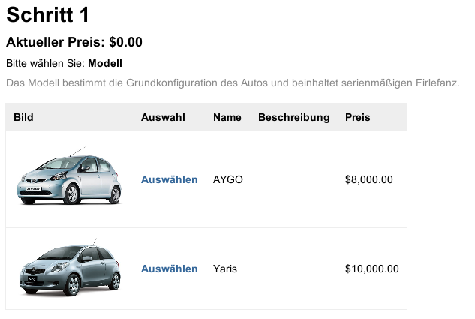
\includegraphics[width=0.8\textwidth]{screenshots/sequence1.png}
\\
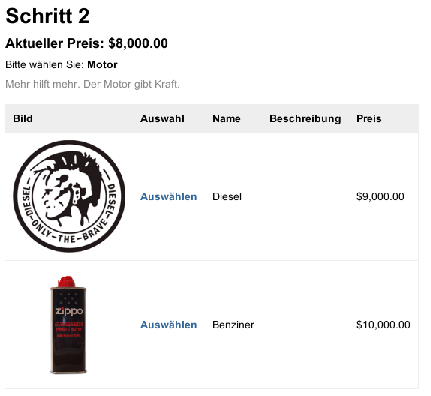
\includegraphics[width=0.8\textwidth]{screenshots/sequence3.png}

\end{document}

% vim: fileencoding=utf8
